\documentclass[conference]{IEEEtran}

\usepackage{graphicx,booktabs,cite,amsmath,stfloats,pstricks,epstopdf,diagbox}
\usepackage{pstricks,pst-node,pst-tree}
\usepackage[caption=false,font=footnotesize]{subfig}
\usepackage{mymacros}

\DeclareGraphicsExtensions{.eps}

\graphicspath{img/}
% correct bad hyphenation here
\hyphenation{op-tical net-works semi-conduc-tor}

\begin{document}

\title{Scenario-based Reasoning \\through Dynamic Decision Networks}

\author{
\IEEEauthorblockN{Patrick de Oude}
\IEEEauthorblockA{
Thales Research and Technology\\
Delft, The Netherlands\\
Email: patrick.deoude@d-cis.nl}
\and
\IEEEauthorblockN{Tom Pepels}
\IEEEauthorblockA{
Thales Research and Technology\\
Delft, The Netherlands\\
Email: tom.pepels@d-cis.nl}
\and
\IEEEauthorblockN{Rik Claessens}
\IEEEauthorblockA{
Thales Research and Technology\\
Delft, The Netherlands\\
Email: rik.claessens@d-cis.nl}
}


\maketitle

% As a general rule, do not put math, special symbols or citations in the abstract
\begin{abstract}
The abstract goes here.
\end{abstract}

\IEEEpeerreviewmaketitle

\section{Introduction}

Decision making in contemporary complex domains, such as large-scale crisis management, Search \& Rescue operations, border security, anti-drug operations etc., can pose an enormous cognitive challenge on the decision maker. Decision makers often need to construct and manage multiple {\em scenarios} regarding the situation description in order to deal with uncertainties that are encountered in these domains. A scenario is a projected or imagined sequence of events describing what could possibly happen (or have happened). By keeping track of the possible scenarios that are compatible with the known information, a decision maker can maintain multiple states of situation awareness. These states are required to be able to make the right decision at the right moment in time. However, the set of possible scenarios may become significantly large in complex real-world applications (typically involving numerous factors and uncertainties), while human cognitive limitations pose restrictions on the number of scenarios that decision makers can effectively handle at any given time. Therefore, to be able to adequately manage a (possibly large) set of scenarios, and  ultimately decide on the information to be presented to decision makers, automated management of scenarios should be addressed.

A scenario can be considered as a narration concerning various events that have materialized (or going to materialize) over time. These events are often causally dependent on each other and can be captured as variables in a causal model \cite{pearl00book}. In \cite{conrado14if} we have shown that these causal models support {\em scoping of states} of scenario variables. Moreover, such causal models can be captured through Bayesian networks (BNs) \cite{pearl88book, jensen07book} to provide a convenient framework to manage a large set of scenarios through: (i) pruning of insignificant scenarios, (ii) updating the scenarios based on new observations and (iii) computing the likelihood of a scenario given the latest information to establish an ordering on the set of relevant scenarios. Additionally, BNs allows what-if exploration where, for example, the likelihood of certain (future) events are computed based on various assumptions about the occurrence of other events of the scenario.

While BNs provide an effective way to manage scenarios it does not allow the actual decisions to be modeled. Neither do they provide recommendations on which decisions to take. In this paper the model {\red which model?} is extended by describing the structure of the decision process. This allows the model to give recommendations regarding decisions under the decision maker's consideration. The extended model is called a {\em decision network} \cite{russell02bn} (also influence diagram or decision graph \cite{jensen07book}). Next to chance nodes decision networks include both decision and utility nodes. such models also support assessment of risk by, for example, computing the worst case scenario considering the utilities in the model.

To facilitate the discussion we consider an example from the maritime security domain about countering a drug smuggling operation by intercepting a drug transport. Such domains, where information becomes available over time, are inherently dynamic. Alongside this, static information, such as Intel about the possible destination of the transport or context information about the area in which the smuggling operation takes place needs to be considered. Given the dynamic nature of this domain, sequential decisions need to be considered. To support incorporation of dynamic and static information as well as sequential decision making we consider {\em dynamic decision networks} \cite{russell02bn, jensen07book}. By casting the scenario model in a DDN we can reason about sequential decisions under various observations, what-if conditions and determine what is the best sequence of decisions to successfully counter the smuggling operation.

In this paper we discuss the methods that are required to do scenario-based reasoning incorporating decisions explicitly in a decision support tool.

{\red What do we expect, are we proposing a planning and simulation tool, (semi-)autonomous mission management, or decision support? I think we should place the proposed solution somewhere, so it is clear what it might be used for. In my view it could be used for all of the above, but it is probably better to focus on one application.}

% In \cite{conrado14if} a method was discussed to manage the set of possible scenarios using Bayesian networks (BNs) \cite{pearl88book, jensen07book}. With the help of BN an estimate of the likelihood of the scenario to unfold can be computed given the evidence that is available at the time. With these likelihoods the set of scenarios can be ranked form most to least likely scenario, which enables the decision maker to focus on the set of most likely scenarios. The method described there did not model the actual decisions that a decision maker could make. In this paper 

%TODO add related work about the use of influence diagrams and secenario based reasoning

% In the BNIn this paper we are going to extend the framework discussed in \cite{conrado14if} with the actual decision

% The models consist only of chance nodes which do not support assessment of risk since this would require utilities to be part of the model. For example, to compute the worst case scenario, which is not necessarily the most likely, information is required about the impact of the scenario. To support risk assessment the framework discussed in \cite{conrado14if} is extended with decision and utility nodes.

% t When time progresses, new evidence might be obtained and the likelihood of the scenarios can be updated.

% When making decisions in complex contemporary applications, e.g. intelligence operations and large-scale crisis management, decision makers often need to construct and manage multiple hypotheses regarding the situation description in order to deal with uncertainties. Hypotheses about a situation's description are commonly referred to as {\em scenarios}. A scenario can be defined as a projected or imagined sequence of events describing what could possibly happen (or have happened). Scenarios can be used to deal with uncertainty by allowing the exploration of diverse descriptions of a given situation (and its possible developments) that are compatible with known information at any given time. Scenarios can thus offer multiple states of situation awareness and help overcome cognitive biases, and as such should ideally explore the whole set of plausible and relevant states of the world. Owing to human cognitive limitations, however, keeping track of all relevant information can become a challenge, even when only a few scenarios are considered.

%TODO add overview of the paper
\section{Causal Models}

%TODO explain the scenario

Maritime drug trafficking is an ongoing problem in the Caribbean sea. Very fast and small vessels, so called go-fasts, are used to transport contraband from Columbia's and Venezuela's coast to Jamaica, Haiti and Dominican Republic to be further transported into North-America. The popularity of a go-fast to be used as a drug trafficking vehicle is due to the go-fast's size, speed and low radar and optical signatures. This makes go-fasts hard to detect and difficult to intercept by often slower coast guard vehicles. Nevertheless, the U.S. coast guard deploys their own go-fasts and helicopters equipped with anti-materiel rifles (AMR) to disable the engine of a running go-fast. 

The main challenge of anti-drug trafficking organizations, such as the coast guard, is to locate the smuggler's go-fast in order to intercept it. There are several type of observations that can be used. Location of the smuggler's go-fast can be determined by radar ($RO$) in case of calm sea or at close range or by visual observation ($VO$). A more recent type of observation is through the use of sonar mounted on buoys in the ocean ($SO$) that can register the typical engine sound of go-fast. Unfortunately, these type of observation might not be available. For radar and sonar the coverage is often limited and, therefore, not always available. A visual observation is only possible if an observer is close enough to report it. Knowledge regarding the location of the smuggler's go-fast allows us to reason about the possible intercept areas. This area can be a location where the smuggler's go-fast currently is or a more strategic position that is believed to be visited by the smuggler at some point in the future. These strategic positions are inferred from Intel collected during the anti-drug operations, for example. There might be Intel that the smuggler needs to refuel at some refueling location along their route ($RA$). This belief is based on Intel about the amount of fuel loaded on board prior to departure ($AF$), the possible destination ($D$) and the possible locations where refueling is possible ($LR$). If there is strong belief that the smuggler is going to refuel at a certain location then that location is a possible intercept area. In Figure~\ref{fig:causal-model} the causal model is depicted that describes the causal influences between these variables. All the variables are listed in Table~\ref{tab:scenario-variables}.

\begin{table}[!ht]
 \centering
 \caption{Overview of scenario variables from the causal model shown Figure~\ref{fig:causal-model}, as well as their semantics.}
 \begin{tabular}[!ht]{rp{4cm}}
\toprule
 Variable & Semantics \\
\cmidrule(r){1-1}
\cmidrule(l){2-2}
$LocationSmuggler$ ($LS$) &
The location of the smuggler's go-fast. \\
$Destination$ ($D$) &
Potential destination to which the smuggler travel. \\
$LocationRefuel$ ($LR$) &
Locations of stationary refuel location in the concerned area of the sea. \\
$Weather$ ($W$) &
Bad weather condition at a certain location $(x,y)$ affecting smuggler's traveling. \\
$RefuelingAction$ ($RA$) &
Occurrence (or not) of a refueling action by the smuggler, as well as its position. \\
$LocationInterceptVehicle$ ($LI$) &
Location of an available intercept vehicle. This could either be coast guard's go-fast or helicopter etc. \\
$InterceptArea$ ($IA$) &
Area where the intercept vehicles can intercept the smuggler's go-fast. \\
$Destination$ ($D$) &
Destination the smuggler are likely to travel to. \\
$RadarObservation$ ($RO$) &
Radar observation of the smuggler's go-fast. \\
$SonarObservation$ ($SO$) &
Sonar observation of the smuggler's go-fast. \\
$VisualObservation$ ($VO$) &
Visual observation of the smuggler's go-fast. \\
\bottomrule
\end{tabular}
%\caption{Overview of scenario variables from the causal graphs in Figure~\ref{fig:causal-graph1} and \ref{fig:causal-graph2}, as well as their semantics.}\label{tab:cpt-example}
\label{tab:scenario-variables}
\end{table}


%TODO define intercept area


% Timely response in Search and Rescue (SAR) operations is most critical in the first few hours after the emergency has taken place. Generally after the initial hours of the incident the chances of finding possible survivors is significantly reduced. Before the actual rescue operation can commence the main challenge is to locate the incident site. In order to locate the incident site the available resources, such as helicopter, planes, ships, search crew, dogs, etc. must deployed as fast as possible at the right location to minimize the localization time. In order to determine initial search location observation that can be used to infer the the possible incident location can be used.

\section{Scenario Modeling}
\label{sec:influence-diagrams}

In \cite{conrado14if} BNs were used to represent a symmetric scenario tree capturing all possible scenarios given the modeled variables and states. The decision maker can use this BN to manage the set of scenarios under consideration using probabilistic inference to do pruning, ranking and what-if exploration. Based on this information the decision maker decides upon a course of action. %by making a decision.
This decision results in an action or a set of actions, which  influence further development of the scenario. For example, sailing the intercept vehicle in the wrong direction, moving away from the smuggler, results in fewer or none possible intercept areas. 

In this paper we extend the scenario reasoning framework discussed in \cite{conrado14if} to include the decisions explicitly. A BN can be extended to include decisions and corresponding utilities. Such a generalized model is called a decision network. In Subsection \ref{sec:bayesian-networks}, we briefly introduce BNs in the described use case. Next, in Subsection \ref{sec:decision-networks}, the described model is extended to include decisions.

\begin{figure*}
\begin{center}
 \subfloat[Causal model of the smuggler scenario\label{fig:causal-model}]{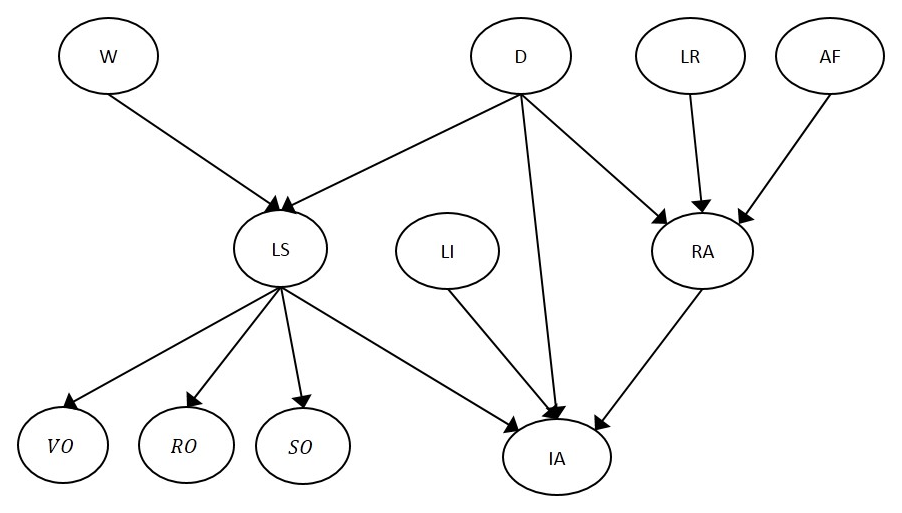
\includegraphics[width=.35\textwidth]{img/causal-model.eps}}\qquad
\subfloat[Decision network based on the causal model shown in Figure~\ref{fig:causal-model}\label{fig:decision-graph}]{ 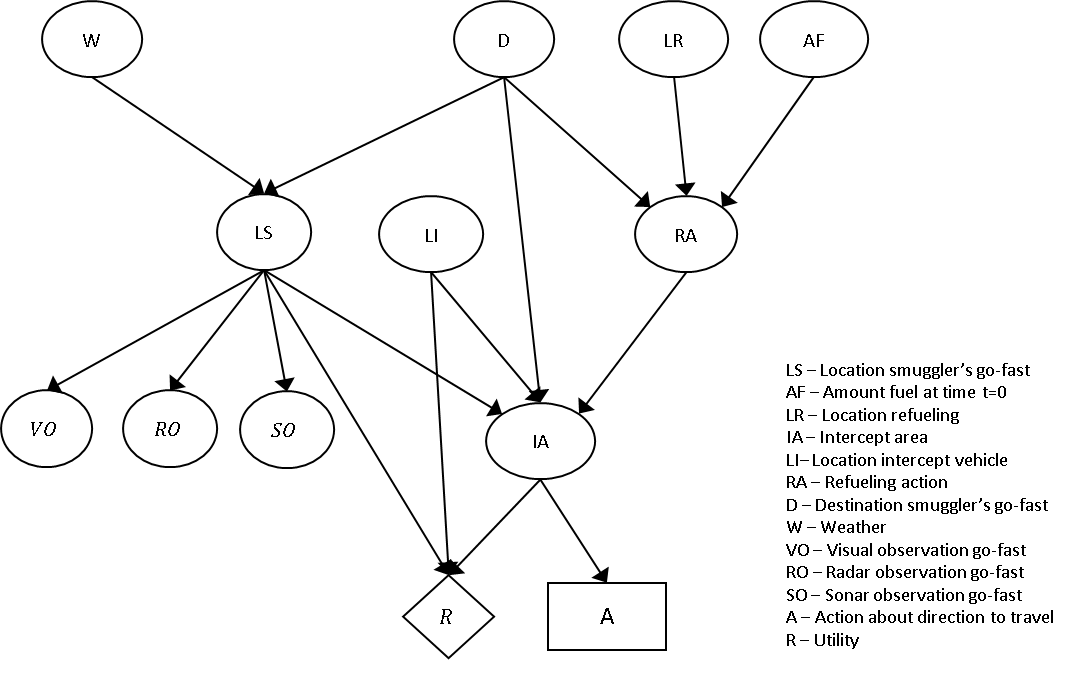
\includegraphics[width=.4\textwidth]{img/decision-network.png}}
 \caption{}
 % decision-graph.eps: 0x0 pixel, 300dpi, 0.00x0.00 cm, bb=-0 -0 424 277
\end{center}
\end{figure*}


\subsection{Bayesian networks}\label{sec:bayesian-networks}

% \begin{table}
% \centering
% \caption{CPT of the discrete CPD $P(LS|D,W)$}
%  \begin{tabular}{c|ccc|c|c} 
% $D$	& \multicolumn{3}{c|}{X} & Y &  Z \\ 
%  \diagbox{$LS$}{$W$} & $(x_1,y_1)$ & \ldots & $(x_n,y_m)$ & & \\
% \hline
%  $(x_1,y_1)$ & 0.1 & \ldots & 1 & \ldots & \ldots \\
%  $(x_1,y_2)$ & 0.9 & \ldots & 0 & \ldots & \ldots \\ 
%  \vdots & \vdots & \vdots & \vdots & \ldots & \ldots \\ 
%  $(x_n,y_m)$ & 0 & 0 & 0 & \ldots & \ldots \\ 
%  \end{tabular} 
%  \end{table}

A Bayesian network (BN) is a probabilistic graphical model that efficiently represents a joint probability distribution (JPD) over a set of random variables \cite{jensen01book,pearl88book}. A BN is represented through a Directed Acyclic Graph (DAG), where each node in the DAG corresponds to a random variable of the JPD. For example, the causal graph shown in Figure~\ref{fig:causal-model} can directly by used to describe a DAG of a BN. Each oval node represents a random variable, and each state of a random variable corresponds to a state of the scenario variable\footnote{Note that, the set of states for the scenario variables (and therefore the range of states for the random variables) is not determined a priori but as the estimation processes take place, as explained in \cite{conrado14if} on scoping of states.}
For each node given its parents in the DAG, a conditional probability distribution (CPD) needs to be specified. For instance, for the variable $LS$ the CPD $P(LS\mid D,W)$ must be specified through a conditional probability table (CPT). 

% Since all scenario variables are discrete, the CPD $P(LS|D,W)$ can be represented through the CPT shown in Figure~\ref{fig:cpt-example}. This CPT expresses that, given destination X and a small amount of fuel on board, the chance that a refueling action takes place (at location 1) is $0.9$, i.e. $P$($A$~=~Yes~at~1$|$$D$~=~X,~$F$~=~Small) = 0.9. For larger amounts of fuel (and the same destination X), it is estimated that no refueling action takes place. Moreover, there is no chance that the refueling action takes place at locations 2 and 3, as these locations are farther than X itself. This example shows that incompatibility of state combinations can simplify the specification of CPTs for scenario variables, as the probabilities of such combinations are zero.

Before the introduction of BNs, probabilistic inferences were performed directly on a JPD defined over several variables. This, however, limited such operations only to JPDs defined over a small set of variables due to the combinatorial complexity. A Bayesian network, on the other hand, exploits conditional independencies between the random variables. Consequently, the JPD can be factorized into CPDs for each variable in the model. 
For example, considering the BN of the causal graph shown in Figure~\ref{fig:causal-model}, the JPD $P(\VV)$ (where $\VV$\footnote{In this section, a single random variable is presented as an uppercase letter and its states as lowercase letters. A set of random variables and of states are shown as bold uppercase and bold lowercase letters, respectively.} = $\{W, D, LS, VO, RO, SO, LR, AF, RA, IA, LI\}$) factorizes into a set of CPDs, \ie


\begin{eqnarray}
P(\VV) = \prod_i P(X_i\mid \Pa(X_i)),  \label{eq:chain-rule}
\end{eqnarray}

\noindent
where $\Pa(X_i)$ denotes the parents of node $X_i$. 

% For the BN in Figure 5a, the JPD is therefore
% 
% \begin{eqnarray}
%  P(W,D,F,A,I) &=& P(W)P(D)P(F)P(A|D,F) \nonumber \\
%   & & \cdot P(I|W,D,A). \nonumber
% \end{eqnarray}


With the help of the chain rule in Equation~(\ref{eq:chain-rule}), a JPD can be represented through its factorization of CPDs, which requires significantly fewer parameters compared to the number of parameters in the JPD. Moreover, by exploiting the conditional independencies between the random variables, efficient exact inference methods can be used, \eg the junction tree algorithm \cite{cowell99bn}.

The likelihood of scenarios can be computed with the help of Equation~(\ref{eq:chain-rule}), given a BN of the causal model that shows the cause-effect relations between the scenario variables. 

% For instance, for the scenario corresponding to the uppermost complete branch of the scenario tree in Figure~\ref{fig:scenario-tree}, i.e. $W$~=~bad, $D$~=~X, $F$~=~Small, $A$~=~Yes at 1, $I$~=~4, the likelihood can be computed as

% \begin{eqnarray}
%  P(W=\text{bad}, D=\text{X}, F=\text{Small}, A=\text{Yes at 1}, I=\text{4}) &=& \nonumber \\
%  P(W=\text{bad})P(D=\text{X})P(F=\text{Small}) & & \nonumber \\ 
%  \cdot P(A=\text{Yes at 1}|D=\text{X},F=\text{Small}) \nonumber \\
%  \cdot P(I=\text{4}|W=\text{bad},D=\text{X},A=\text{Yes at 1}). \nonumber
% \end{eqnarray}

  
Moreover, one of the main strengths of BNs is the possibility to perform predictive or diagnostic inference based on a given set of evidence denoted by $\E$. For example, the belief over the position of the smuggler, \ie variable $LS$, can be updated when for example evidence is obtained about the destination $D$. In this case we could compute the posterior probability $P(LS\mid \epsilon)$, where $\epsilon = \{D=destX\}$.


% in the second phase of the example the weather is observed, i.e. $\E = \{W = \text{bad}\}$. With this observation, the likelihood of the scenarios can be updated by computing $P(\vv|\E)$, where $\vv$ is a configuration of random variables states corresponding to a given scenario. Note that all scenarios with $W = \text{good}$ will get zero probability due to the observation. Assigning zero probabilities to scenarios after an observation update corresponds to pruning of scenarios based on evidence.

% Also in the second phase of the example (whose BN is shown in Figure~\ref{fig:bn-example}), a new variable $R$ is added to the model to capture the received refuel report. The model needs to be updated by specifying the CPD $P(R|A)$ as well. The new JPD $P(W,D,F,A,I,R) = P(W)P(D)P(F)P(A|D,F)P(I|W,D,A)P(R|A)$ can be used to re-compute the likelihood of the scenarios, given the occurrence of the refueling report at position 1.




\subsection{Decision Networks}\label{sec:decision-networks}

A {\em decision network (DN)} (also influence diagram or decision graph \cite{russell02bn,howard84rpada,jensen07book}) is a concise graphical and mathematical representation of a decision problem. For example, the BN described in the previous section can be extended into the decision network (DN) shown in Figure~\ref{fig:decision-graph}. This DN consists of the same chance nodes as in the causal model in Figure~\ref{fig:causal-model} plus a decision node $B$ and a utility node $U$. A decision node represents possible actions the decision maker can take. In this case the actions are the different bearings the intercept vehicle can travel, such as North, East, South-west, etc. Next to the decisions we model the desirability of the states we end up in after taking an action. This desirability is modeled through the utility node and is dependent on the location of the intercept vehicle and areas. It is desirable that the intercept vehicle is near or at the location of the intercept areas prior to arrival of the smuggler, such that we are able to intercept the smuggler. Thus, the preference of the decision maker can be captured through a utility function that uses the position of the intercept vehicle and intercept areas as arguments.

The location of the intercept vehicle\footnote{In this section we assume there is only a single intercept vehicle} and the smuggler's go-fast constitute a state $s$ in a set of states $\S$ defining the smuggler's domain. However, due to partial observability of the current state, the decision maker (also called agent in decision theoretic literature) has to maintain a belief $P(\S = s \mid  a, \epsilon)$ over the possible states it might be in given an action $a$ and evidence $\epsilon$. The reason for this is that the position of the smuggler is not directly observable after an action $a$, but needs to be estimated from observations $\epsilon$, such as radar, sonar, visual observations or Intel about a possible destination or refueling location (see also causal model in Figure~\ref{fig:causal-model}). Since the agent does not know in which state it is it needs to compute an expected utility based on the utility function $U(s)$ capturing the preferences of the decision maker:

\begin{eqnarray}
 EU(a|\epsilon) = \sum_{s'}P(\S = s'\mid a, \epsilon)U(s')
\end{eqnarray}

With the help of the expected utility $EU(a|\epsilon)$ the best action $a^*$ can be computed with:

\begin{eqnarray}\label{eq:meu}
 a^* = \argmax_a EU(a\mid \epsilon)
\end{eqnarray}

Equation~\ref{eq:meu} presents two challenges we need to address in order to compute the best action $a^*$, namely the estimation of $P(\S = s'|a, \epsilon)$ and the computation of the utility using the utility function $U(s')$.


% 
% 
% {\red needs to be reworked - Patrick}
% 
% The BN described in the previous section can be extended into the decision network (DN) shown in Figure~\ref{fig:decision-graph}. This DN consists of the same nodes as in the causal model in Figure~\ref{fig:causal-model} plus a decision node $D$ and a utility node $U$. A decision node represents possible actions the decision maker can take. In this case the actions are the different directions the patrol ship can travel, such as North, East, South-west, etc. The utility node, on the other hand, represents the utility function where the parents of the utility node, i.e. $\{LS,LP,IA\}$, are the arguments of this function:
% 
% \[
%  U(LS,LP,IA) = -\alpha d(LS,LP) - (1-\alpha) d(IA,LP),
% \]
% 
% where $d(X,Y)$ is the distance between $X$ and $Y$ and $\alpha$ is a value between $[0,1]$ that is used to control the importance of either $d(LS,LP)$ or $d(IA,LP)$. In case $\alpha=1$ the utility function is $U(LS,LP,IA) = -d(LS,LP)$ and therefore solely based on the distance between the smuggler's boat and the patrol ship, while $\alpha=0$ the utility function is solely based on the distance of the patrol ship and the intercept area. The choice of $\alpha$ should be based on the information that is available. If more information is available that could help to locate the smuggler's go-fast then we want to weight  $d(LS,LP)$ more by using a higher $\alpha$ value. A higher utility is obtained when the patrol ship is either closer to the smuggler's location or to an intercept area (where eventually the smuggler should travel to).

% In order to evaluate the different decisions modeled in a DN the impact of the decision's consequences need to be measured. The consequence of a decision is measured through a utility node. For example, we need to drive to work either via route A or route B in the shortest amount of time. Clearly in this case the utility is based on the amount of time required to travel to work and the route that results in the lowest amount of time gets a higher associated utility value. In Figure~\ref{fig:decision-graph} an example of a DN is shown with a single decision variable (square node) and utility variable (diamond node) together with several random variables (oval nodes). Since a DN is generalization of a BN we start discussing BNs first.

\begin{figure*}[!t]
\begin{center}
 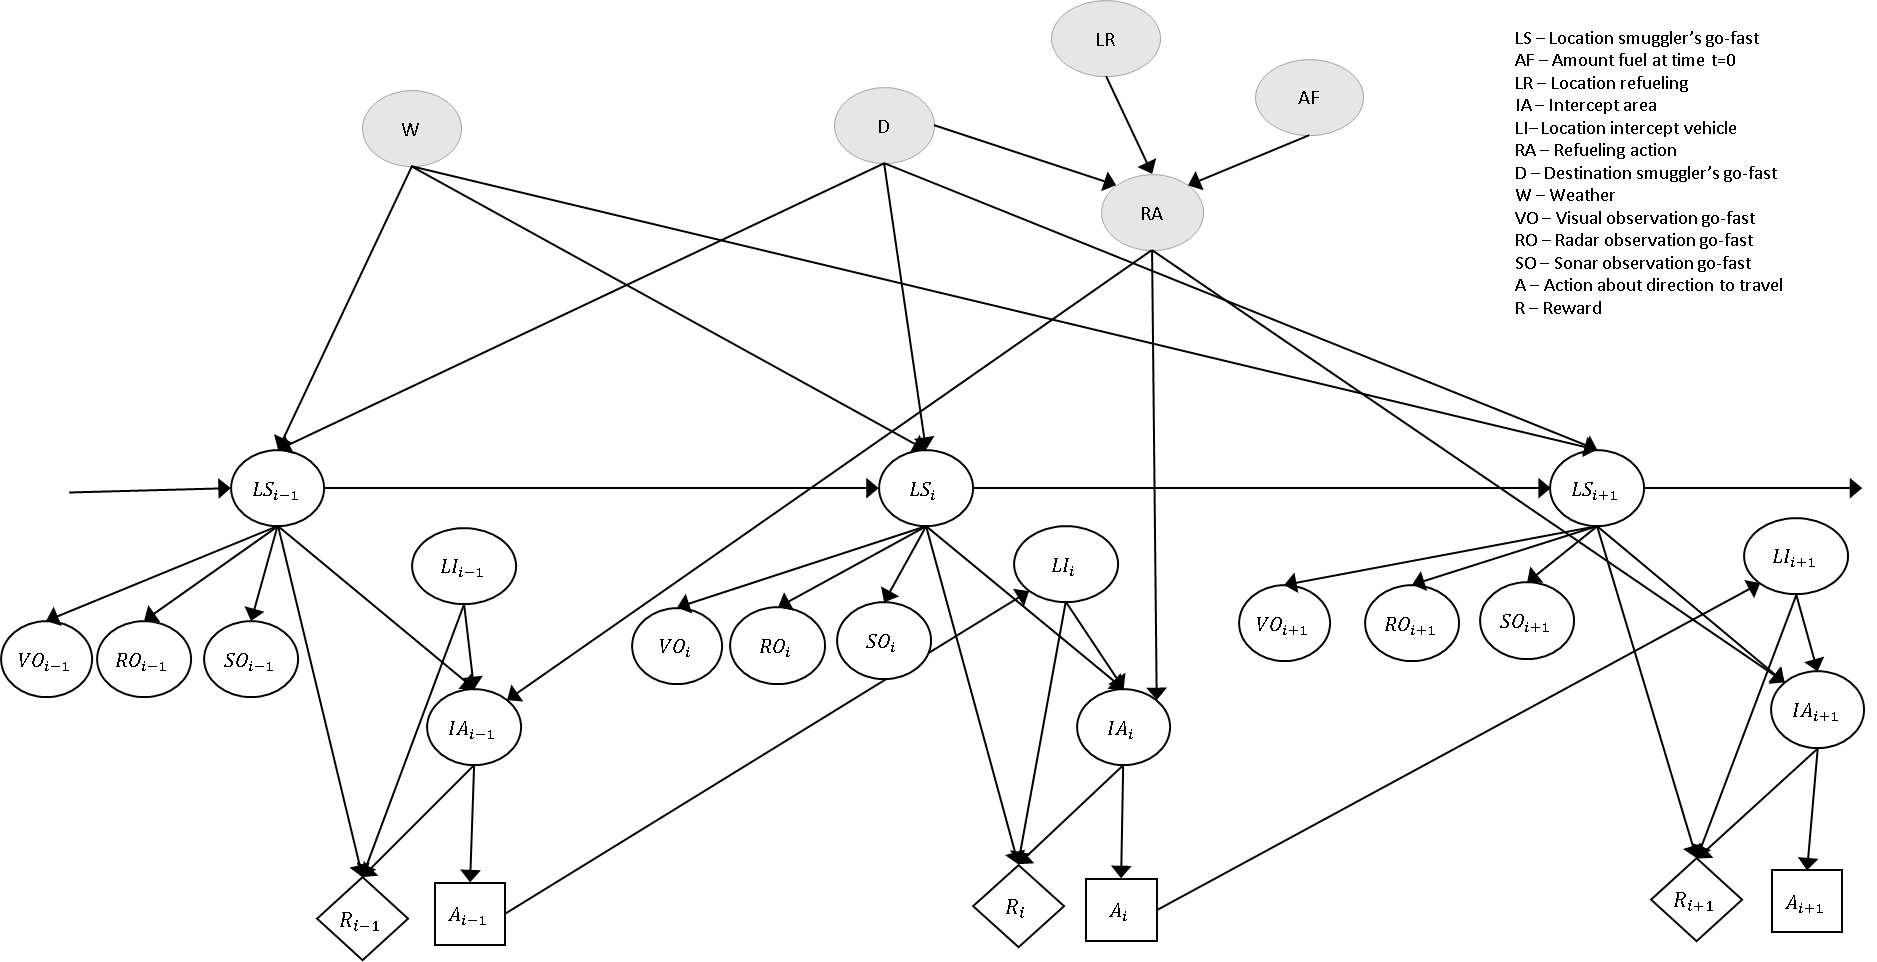
\includegraphics[width=.95\textwidth]{img/dynamic-decision-graph.png}
 \caption{Dynamic decision network of the decision network shown in Figure~\ref{fig:decision-graph}.}\label{fig:ddn} 
\end{center}
\end{figure*}


\subsection{Dynamic Decision Networks}
\label{sub:dyn-dec-net}

In the Figure~\ref{fig:decision-graph} a decision network was shown for a so-called \emph{one-shot} decision. However, intercepting a smuggler that is actively trying to prevent capture governs an environment that is very dynamic. In such environments a one-shot decision is not sufficient and sequential decision making is required to be able to reason about scenarios relevant for intercepting the smuggler. In Figure~\ref{fig:ddn} a {\em dynamic decision network (DDN)} is shown based on the one-shot DN shown in Figure~\ref{fig:decision-graph}. A DDN consist of a Dynamic Bayesian Network (DBN) \cite{murphy00book} and a set of decision and utility nodes. A DBN is a BN discussed in Section~\ref{sec:influence-diagrams} {\red dat is deze sectie} and describes a temporal probabilistic model that allows reasoning about variables over time. In a DBN, transition probabilities for dynamic variables are to be specified. For example, in Figure~\ref{fig:ddn} the transition probabilities for the location of the smuggler are to be specified. Note that, there is no direct link between the position of the intercept vehicle $LI_i$ and $LI_{i+1}$ in two consecutive time slices, because we assume that the location fo the intercept vehicle is always known. This means that the variable $LI_i$ can be observed in each time slice.

In the DDN shown in Figure~\ref{fig:ddn} we distinguish between two types of chance variables, namely dynamic variables that change over time, shown as white oval nodes, and static variables that are time invariant during the smuggling operation, shown as gray oval nodes. Observations for time invariant nodes are typically coming from Intel. For example, Intel can be acquired about the possible destination of the smuggler. Moreover, in this model we assume that the state of the weather ($W$) at a certain location remains unchanged, \ie once the weather is observed its state is assumed not to change.

Because the location of the smuggler is not directly observable, the model depicted in Figure~\ref{fig:ddn} is considered a Partially Observable Markov Decision Process (POMDP). The location of the smuggler needs to be estimated through observations such as radar ($RO_i$), visual ($VO_i$) or sonar ($SO_i$) observations. Additionally, information regarding weather $W$, and destination $D$ can be used to estimate the location of the smuggler.

\subsection{Partially Observable Markov Decision Process}
\label{sub:pomdp}
{\red connect this to the previous section - Tom \& Patrick}

A Markov Decision Process (MDP) \cite{bellman1957dynamic,mdp} describes synchronous interactions between an agent and the world. MDPs are used to model sequential decision making problems in which the current state determines the complete dynamics of the world. At each time-step $t$, an agent takes an action, changing the state and collecting a reward. The MPD model can be extended to describe multi-agent decision-making without changing the formal description. An MDP is formally described as the tuple $\langle\S,\mathcal{A},\P,R,\gamma\rangle$, where:

\begin{itemize}
\item $\S$ is the set of states of the world. The state space can be factored, meaning that it is represented by a discrete set of state variables, described as a vector $\left(X_1,\ldots,X_n\right)$ where each variable $X_i$ can take on a value in its domain,
\item $\mathcal{A}$ is the set of possible actions. In the case of a multi-agent problem $\mathcal{A}$ represents the joint actions $\A_{m} = \A_1\times\ldots\times\A_n$ of all $n$ agents under consideration,
\item $\P:\S\times\mathcal{A}\to\P(s'\mid a,s)$ is the state transition function \ie the probability of moving to state $s'$ given that action $a$ was performed in state $s$,
\item $R:\S\times\mathcal{A}\to\mathbb{R}$ is the reward function, which maps each state-action pair to a real reward,
\item $\gamma$ is the discount factor, which represents prioritizes present over future rewards.
\end{itemize}

In the case of MDPs the assumption is made that an agent can fully observe the world, as is the case in for instance games of complete information like Chess or Checkers. However, in many real-world domains, the state of the world is not fully observable, and the agent cannot determine the state it is in with complete accuracy. To represent this uncertainty over the agent's current state and observations, the MDP model can be extended to the Partially Observable MDP (POMDP) \cite{aastrom1965optimal,pomdp} such that: 

\begin{itemize}
\item $\S,\mathcal{A},\P,R,$ and $\gamma$ describe the MDP,
\item $\mathcal{O}$ is the set of possible (joint) observations,
\item $O:\S\times\mathcal{A}\to\P(o\mid s)$ is the probability of observing $o$ in state $s$. 
\end{itemize}

A history describes a sequence of actions and observations, $h_t = \{a_1, o_1, \ldots, a_t, o_t\}$. In a POMDP, agent(s) maintain an internal {\it belief state} $\B = P(s_t\mid  h_t)$, in which the probability distribution over the possible states are summarized given history $h_t$. The agents' action selection policy $\pi(h,a)$ determines the probability distribution $P(a_{t+1}\mid h_t)$ over available actions, given the current history, and the value function $V_{\pi}(h)$ is the expected {\it return} from state $s$ when following policy $\pi$. The return $R_t = \sum\nolimits_{k=t}^{\infty} \gamma^{k−t}r_k$ is the total discounted reward accumulated from time $t$ onward. In any POMDP there is at least one optimal policy $\pi*(h, a)$ with the optimal value.

POMDP's are harder to solve exactly than MDP's, suffering from both the {\it curse of dimensionality} as well as the {\it curse of history}. Therefore, they require approximate methods to be used in real-world problems \cite{pineau2006anytime}.

In Section \ref{sec:scenario-based-dm} we will describe a configuration of a POMDP in order to introduce an approach to sequential planning and decision-making under uncertainty in the smuggler use case. 

% Making decisions based on a POMDP defined in the previous section
%\begin{figure}[t]
%\begin{center}
% 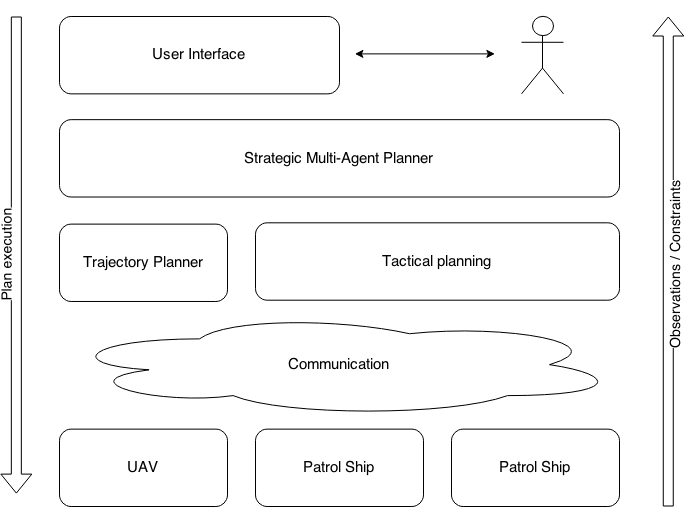
\includegraphics[width=.44\textwidth]{img/planning_archi.png}
% \caption{Architecture of multi-layered planner.}\label{fig:planning-archi}
%\end{center}
%\end{figure}

\section{POMDP for the Drug Trafficking Domain}
\label{sec:scenario-based-dm}

In Section \ref{sec:influence-diagrams} models are used to describe a formal reasoning method about possible future states of a drug trafficking event. Based on these models, we can explore possible futures and strategies to create a robust plan of action. The goal of this section is to define the elements of the POMDP model as described in Subsection \ref{sub:pomdp}, which we will use in Section \ref{sec:ma-dec-mak} to establish and rank decisions.

\subsection{Planning Under Uncertainty}
\label{sub:plan-uncert}

To scope the definition of our problem, we make the assumption that the locations of all friendly agent is available. Moreover, we assume that two-way communication with the agent is possible, such that commands can be sent, and observations received. The proposed methods can nonetheless be extended to environments where agents can not share their observations. In this case, a \emph{decentralized} POMDP (DEC-POMDP) \cite{dec-pomdp,oliehoek2008optimal} model is to be defined.

Based on the decision network depicted in Figure \ref{fig:decision-graph} an exploration of possible plans should be generated to explore which course of action is the most likely to capture the smuggler. In this section, the individual elements of the POMDP are defined in order to use an algorithm to generate plans for the intercept vehicle. The state $\S$ represents the possible locations of the intercept vehicle $(LI_i)$. Moreover, we define a particle filter to map the agent's belief over the possible locations of the smuggler $(LS_i)$ in which the context of the problem has an influence on the location of the smuggler. Variables such as the expected destination $(D)$, refueling actions $(RA)$ and external factors such as the weather $(W)$ all influence the belief over the location of the smuggler. The actions $\A$ represent the he intercept vehicle's decisions $(A)$. The agent receives a reward $r$ only when the smuggler is captured. This can be defined as the fact that the agent is in the direct vicinity of the smuggler. Lastly, observations $\mathcal{O}$ map to the evidence nodes $(VO_i), (RO_i), (SO_i)$ in the decision network.

The following subsections define an abstract model of the domain in which high-level decisions can be generated.

\subsection{Problem Representation}
\label{sub:problem-rep}

Maritime security situations may play out over a sizable area. Based on the situation, the concerned region can span over dozens of kilometers. Planning on a (near-)continuous state space would soon become intractable based on the number of hidden locations for the smuggler and action spaces for the intercept vehicles. Therefore we propose a framework in which an area of interest is factored into discrete elements. Based on the surface-area and the required resolution of the mission, a region is selected on a geographical system that is divided into discrete cells of a desired resolution. Higher resolutions result in more fine-grained plan at the cost of computational complexity.

The state represents the location of the intercept vehicle under consideration for the planner. The model can be extended to represent multiple agents, in which each agent $\psi_i\in\Psi$ occupies a single location defined by the underlying geographical area in which the scenario takes place.

Given a factored state space $S = \left(X_1, \ldots, X_n\right)$, the domain of each variable $X_i$ can be defined as a single agent. Each variable's domain is restricted based on the underlying geographic characteristics \ie boats can only occupy a location on water. Moreover, political borders and no-fly zones can further restrict the domain of each variable.

Similarly, the action space is factored based on the discretization of the state space. Suppose the state space is factored into square grids, then the possible actions for agents consist of $a\in\left\{n, nw, w, sw, s, se, e, ne, \o\right\}$ where $\o$ represents taking no action. Based on the speed of each agent, actions are performed in specific intervals, where each action relocates the agent to an adjacent cell. Using such atomic actions, a set of waypoints can be defined to represent a plan. Waypoints are generated by repeatedly selecting the same action until the plan requires movement in a new direction. For instance, an action sequence for a given agent $a_i: n, n, n, n, w, w, w$ can be transformed to two waypoints, the first four cells north, and the second three cells west to the first.

The space of observations $\mathcal{O}$, in the smuggler's case is small. The smuggler is either observed, or not observed. We identify two types of observations:
\begin{itemize}
\item based on the sensor payload of each agent, an observation model describes the observation footprint, and the noise-level of observations,
\item external observations, unrelated to the state and actions of the agents may also occur. These observations can be modeled as evidence in the BN defined in Section \ref{sec:influence-diagrams}.
\end{itemize}

\subsection{Belief Filtering with Context}
\label{subsec:belief-filter}

In the defined state representation, the locations of the friendly agents are assumed to be known at each point in time. This assumption is based on the availability of GPS localization and wireless communication techniques. However, the location of the smuggler is unknown to the agents. Given that the goal of the multi-agent plan is to locate, track and capture the smuggler, respectively, the combined set of agents needs to maintain a belief over the current location of the smuggler's go-fast.

The challenge in the targeted domains is often that available sensors do not provide full coverage of the area of interest and therefore, observations are sparse, of low quality and disparate in nature. The belief of the target's true location is a probability distribution over his possible location. Generally, exact computation of this distribution is infeasible, so a suitable approximation algorithm is required.

A common technique for target tracking is Particle Filters (PF) \cite{Blackman1999}. The PF-algorithm makes use of a set of particles, representing possible locations of the target. A particle's so-called importance factor represents the likelihood of that particle being correct. The distribution of the set of particles gives a measure for the uncertainty about the target's true location.

Given the current scenario it is possible to improve the PF's tracking performance, by ruling out particles that - based on the scenario - cannot be correct \cite{deOude2014}. For instance, given the DDN in Figure \ref{fig:ddn}, there are two variables that influence the location of the smuggler ($LS$): $W$ and $D$. Assume that at some moment after receiving a specific piece of intel, the destination of the smuggler ($D$) becomes known. This information can be used to predicts possible routes of the smuggler to this designated location. Consequently, these routes can then be used to improve the planning.

\subsection{Planning With Multiple Agents}
\label{sub:plan-mult-ag}

As described, the definition of our POMDP can be extended to include decision-making by multiple agents. This results in an altered problem definition. Nonetheless, the models to be used can be trivially extended by considering joint actions and observations by the set of agents.

Locating and capturing the smuggler by multiple agents requires some form of centralized coordination. The team can be heterogeneous in the sense that different agents have different levels of autonomy, capabilities, and payloads. For example, we may have the availability of two UAV's with infrared sensors, and four armed, human operated patrol boats. Given this task force, several distinct but reliant tasks can be distinguished:
\begin{itemize}
\item locating the smuggler based on its most likely location and observations,
\item tracking the location smuggler after is was located,
\item capturing the smuggler by strategic positioning of patrol boats.
\end{itemize}
Planning these tasks requires cooperation between the agents. Therefore, a joint strategy for the execution of such a plan, based on the uncertain knowledge provided by prior knowledge and observations may play a large role in the success of such missions. Moreover, exploring possible future scenario's based on the expected behavior of the smuggler may offer new insights for human operators.

\section{Planning and Decision-Making}
\label{sec:ma-dec-mak}

Making decisions in uncertain situations is a complex strategic task. In circumstances where situational knowledge and observations are sparse it is hard for humans to predict and rank all possible outcomes in order to develop a robust plan. Therefore, using the described definition of the smuggler case as a POMDP, our goal is to find a joint strategy that minimizes the probability of escape for the smuggler. Online planning offers the capability of establishing a plan that (i) immediately generates an ongoing strategy, (ii) which improves over time, and (iii) can manage incoming observations, sudden constraints, and changing situations. 

Using a forward search technique, the current belief is used to form an approximation of the optimal value function. Generally, online planning algorithms for POMDPs use a point-based value iteration \cite{pineau2006anytime,ross2008online}, generating and traversing a search tree in a heuristic best-first order. However, these techniques are only efficient if the POMDP is either compactly factored, or has a small state space. Moreover, these techniques cannot be interrupted to return a policy at anytime, rather, they require the search to be fully completed in order to return a policy. Lastly, introducing new knowledge such as new constraints or intelligence would require outright re-planning.

\subsection{Monte-Carlo Tree Search}
\label{sub:mcts}

Using Monte-Carlo methods for online planning is an active branch of research in artificial intelligence \cf \cite{browne2012survey}. {\it Monte-Carlo Tree Search} (MCTS) \cite{coulom2007efficient,kocsis2006bandit} is a simulation-based best-first search technique for decision-making problems. MCTS has shown to improve performance in various domains such as games, planning, and scheduling \cite{browne2012survey}. Often, these types of domains can be represented as a form of MDP or POMDP, and new research has shifted focus to adapting MCTS specifically to POMDP domains \cite{silver2010monte,Feldman12BRUE}. 

In MCTS, nodes are evaluated based on the results of numerous Monte-Carlo simulations. As such, a generative model of the domain (\ie simulator) is required, to sample possible futures. Instead of performing an exhaustive search, MCTS grows a search tree incrementally over time. As a result, the constructed tree can be queried to return an action at \emph{anytime}. At all times, each node in the tree maintains a visit count $n(s, a)$, and average sampled value $Q(s, a)$ for each action. $Q(s, a)$ represents an estimate of the value of the (partial) policy represented by the node's descendants. Simulations are performed by sampling states in the tree from the root to a leaf, consequently growing the tree by \emph{expanding} the sampled leaf with a follow-up action. Each simulation consist of two parts, 1) the \emph{selection} step, where actions which are part of the tree are selected and simulated according to the {\it selection policy}, and 2) the \emph{rollout} step, for nodes currently outside the tree, where moves are played according to a \emph{rollout policy}. After each rollout, its result is backpropagated from the expanded leaf to the root, incrementing $n(s,a)$, and updating $Q(s,a)$ with the sampled result for each node along the selected path in the tree.

During the selection step, a policy is required to explore the tree to choose promising actions. The UCT algorithm~\cite{kocsis2006bandit} is derived from the UCB1 policy \cite{auer2002using}. UCT considers each action as part of a multi-armed bandit, and minimizes the number of suboptimal actions sampled. Consider a node $p$ with children $I(p)$, then the policy determining which child's $i$ action to select is defined as:
\begin{equation}
\label{eq:uct}
i^* = argmax_{i \in I(p)}\left\{ Q(s,a) + C \sqrt{ \frac{\ln{n(s)}}{n(s, a)}}\right\},
\end{equation}
where $n(s)$ and $n(s, a)$ are the visit counts of the current node and its child, respectively. $C$ is the exploration constant to tune. Commonly, the \emph{rollout policy} selects actions uniformly random. However, using heuristics or domain knowledge can greatly improve the quality of the recommended decisions \cite{browne2012survey}.

\begin{figure}
\begin{center}
 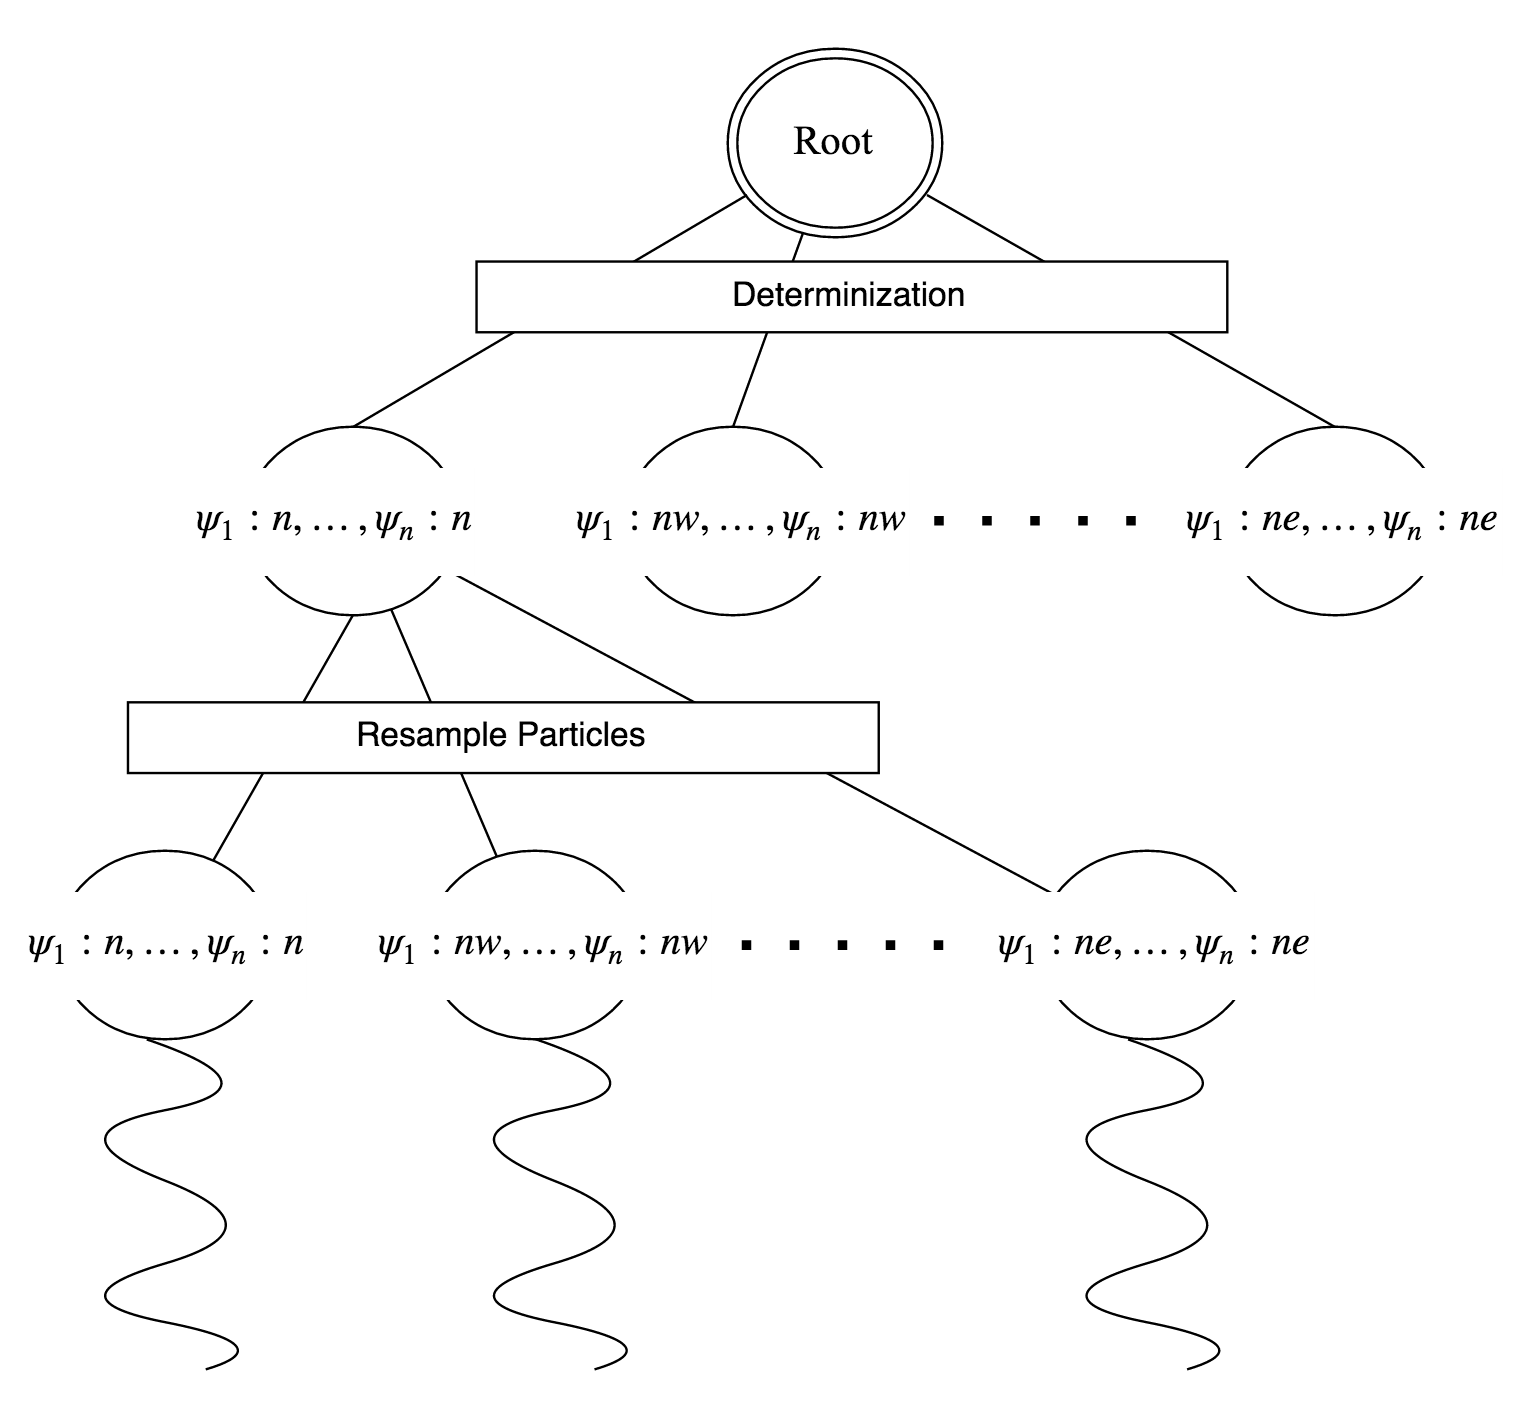
\includegraphics[width=.44\textwidth]{img/searchtree.png}
 \caption{Example MCTS Search procedure with 3 actions and two observations. $a_i$ represent joint actions, $o_i$ represent joint observations. The labels describe the individual steps in a single iteration.}\label{fig:searchtree}
\end{center}
\end{figure}

The final plan for each agent can be retrieved from the tree by following the \emph{critical path}, \ie the path with the highest average reward. After performing a real action and observation, the current tree's root is replaced by the corresponding node. As such, the current information in the tree is maintained, while discarding all subtrees irrelevant to the current state.

\subsection{Partial Observability in MCTS}
\label{sub:pomcts}

The standard procedure in MCTS is to build a tree consisting of states $s$ and corresponding actions $a$. However, in partially observable domains, the exact state is unknown to the search, and therefore the simulator. Complications arise because different actions can be available in different states, or different observations may occur during consecutive search iterations. The straightforward approach to handle partial observability in search is to \emph{determinize} the state at each search iteration. When determinizing, search is conducted over a randomly initiated observable instance of the problem. During search, multiple versions of the tree are built for each individual determinization, and average utilities over all determinizations are used to make a recommendation. However, this approach this leads to the problems of \emph{strategy fusion} and \emph{nonlocality} \cite{cowling2012information}.

Silver and Veness, and Cowling and Powley \cite{silver2010monte,cowling2012information}, propose to maintain a value over histories $V(ha)$ instead of states for the nodes in the tree. As such, the search tree contains both action nodes and related observation nodes instead of merely nodes that represent states. In the drug trafficking case, the sparsity of observations  limits the branching factor, either the smuggles is observed, or unobserved. Moreover, Silver and Veness propose to use a particle filter to maintain the current belief state between actions. The state to use in every MCTS simulation is randomly sampled (\ie determinized) from the current belief at the start of each simulation. During simulation, the particle filter is updated based on simulated actions and observations. Their technique was shown to improve planning performance in large POMDPs. The overall PO-UCT procedure as proposed in \cite{silver2010monte}, is depicted in Figure \ref{fig:searchtree}. 

Simulated actions by the smuggler are thus not incorporated in the tree. Rather, they are determined based on the smuggler's rollout policy $\pi_{smuggler}$. This policy may also incorporate information not visible to the smuggler, such as the positions of intercept vehicles. In order to model the problem as a game, in which the smuggler actively attempts to avoid capture, the tree can include the smuggler's actions and search would be performed as MiniMax.

\section{Discussion}
\label{sec:discussion}

To summarize the methods and models presented in the previous sections we discuss the expected challenges for multi-agent planning in the smuggler's use case. 

The dynamic decision network described in Subsection \ref{sub:dyn-dec-net} was translated into a POMDP as described in Section \ref{sec:scenario-based-dm}. The general approach to generating decisions for large POMDPs was then described in Subsections \ref{sub:mcts} and \ref{sub:pomcts}. As such, we can define a general solution combining decision networks, POMDPs and MCTS for decision making in the described domain. 

The expected challenges to be encountered are as follows:
\begin{itemize}
\item Sparse initial knowledge may result in only a rough approximation of the smuggler's location. As such, finding a plan that is guaranteed to intercept the smuggler may be difficult.
\item Considering multi-agent planning, the number of joint actions may be huge. For instance, considering the action space defined in Subsection \ref{sub:problem-rep} with four agents, this results in a branching factor of $\left\vert\A\right\vert  = 9^4 = 6561$. This problem can be countered by using heuristics in the search process, such as \emph{progressive widening} \cite{chaslot2008progressive}. Another reduction in the action space may be achieved by removing reverse actions from the search \cite{realtime2014}. 
\item The behavior of the smuggler should be realistically simulated. Due to the large state space, it is not realistic to consider the smuggler's actions as part of the search. Rather, a simulation policy should select realistic moves for the smuggler based on his destination, while leaving room for small variations.
\item A random rollout policy for the intercepting agents is not sufficient. Instead, during rollouts, agents should select actions using some heuristic policy.
\end{itemize}
{\red add to this list - all}

%\section*{Acknowledgment}

\bibliographystyle{IEEEtran}
\bibliography{tombib,BNbib}

% that's all folks
\end{document}